\documentclass{article}
%\usepackage{fullpage}
\usepackage{a4wide}
\usepackage{listings}
\usepackage{url}
\usepackage[pdftex]{graphicx}
\usepackage{float}
%\usepackage{color}
\usepackage[unicode,colorlinks,hyperindex,plainpages=false,pdftex]{hyperref}

\lstset{
basicstyle=\footnotesize,       % the size of the fonts that are used for the code
%breaklines=true,        % sets automatic line breaking
%breakatwhitespace=false,    % sets if automatic breaks should only happen at whitespace
%escapeinside={\%*}{*)},          % if you want to add a comment within your code
escapechar=\&,
}

\begin{document}

\title{How to setup Contiki on AVR Raven with ATMega1284P}
\author{Josef Lusticky}
\date{June 17, 2012}

\maketitle

For using copy \& paste, ASCII text files can be generated
using {\it{detex}} or {\it{make text}} command.
All photos can be found in full size in {\it{img}} directory.

\section{Preparation}
In this guide we assume the following equipment:

\vspace{0.2cm}

{\textbf{Hardware:}}
\begin{itemize}
	\item PC running Linux (any other OS should also work, but the GNU software is required)
	\item AVR Raven with ATmega1284P - \url{http://www.atmel.com/tools/AVRRAVEN.aspx}
	\item Two LR44 batteries or external power supply for AVR Raven
\begin{figure}[H]
  \centering
  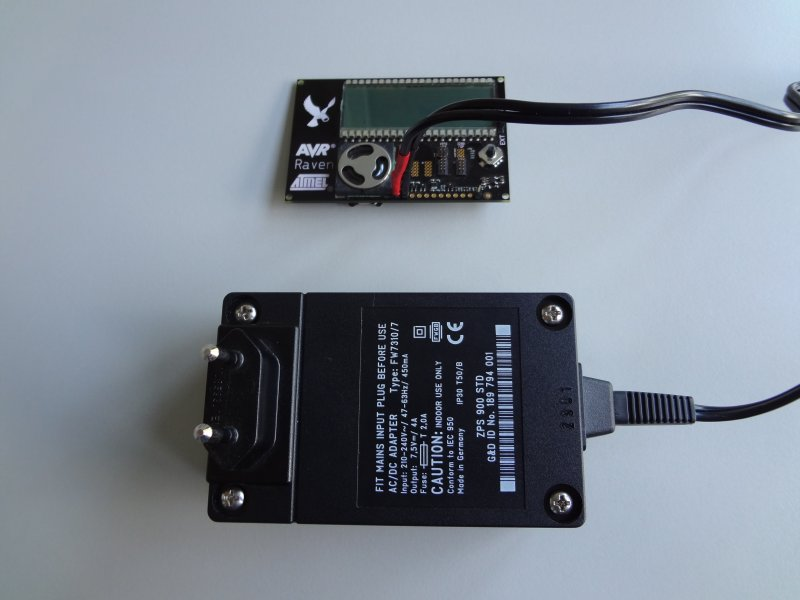
\includegraphics[width=9cm,keepaspectratio]{smallfig/DSC02594-small.jpeg}
  \caption{External power supply connected to AVR Raven}
\end{figure}
	\item AVR Dragon programer - JTAG connection to AVR Raven - \url{http://www.atmel.com/tools/AVRDRAGON.aspx}
	\item USB A/B Cable for connecting PC with AVR Dragon
	\item Optional RZ USB stick for communication between PC and AVR Raven
	(mandatory for network communication) - \url{http://www.atmel.com/tools/RZUSBSTICK.aspx}
	\item Optional Router Advertisement Daemon - radvd (for automatic IPv6 configuration)
\end{itemize}

NOTE: Two AVR Raven devices and one RZ USB stick can be ordered as
evaluation starter kit called RZ Raven - \url{http://www.atmel.com/tools/RZRAVEN.aspx}

%----#--SETUP AVR Raven connection + Photos -> HTML
% As last connect AVR Raven to power.

\vspace{0.5cm}

{\textbf{Software:}}
\begin{itemize}
	\item Contiki source code - zip version 2.5 from\\
	\url{http://sourceforge.net/projects/contiki/files/Contiki/Contiki%202.5/contiki-2.5.zip/download}
	or after cloning git repository by issuing {\it{git checkout 2.5}}
	\item Programmer (flasher) for AVR - avrdude - \url{http://www.nongnu.org/avrdude/}
	\item GNU AVR toolchain - avr-libc 1.6.8, binutils-avr 2.20.1, gcc-avr 4.3.5 -
	newever versions may not work with Contiki version 2.5. % !TODO - how does it look.
\end{itemize}

If we want to interface with the hardware as non-root user, we need to configure udev.
Put the following line to file under {\it{/etc/udev/rules.d/99-avrdragon.rules}}:
\begin{lstlisting}
SUBSYSTEMS=="usb", ATTRS{idVendor}=="03eb", ATTRS{idProduct}=="2107", MODE="0666"
\end{lstlisting}
The idVendor and idProduct can be determined from the output of lsusb command when the hardware is connected.
The mode 0666 sets this device writable for all users.
The udev or a whole PC might need to be restarted to apply changes.


\section{Compiling and flashing}
After everything from step 1 installed and connected, we can navigate to a Contiki project and flash it to AVR Raven:
\begin{lstlisting}
change to project directory:
	&\textdollar& cd contiki/examples/hello-world

select target platform and save our choice to Makefile.target file:
	&\textdollar& make TARGET=avr-raven savetarget

compile the project for our saved target avr-raven:
	&\textdollar& make
\end{lstlisting}
Now we have the hello-world project compiled for avr-raven target.

To see all available target platforms issue the following command:
\begin{lstlisting}
	&\textdollar& make targets
\end{lstlisting}

Next we need to upload our compiled project to AVR Raven.
The connection for flashing ATmega1284P CPU is shown bellow.
Do not forget that AVR Raven must be powered while flashing.
\begin{figure}[H]
  \centering
  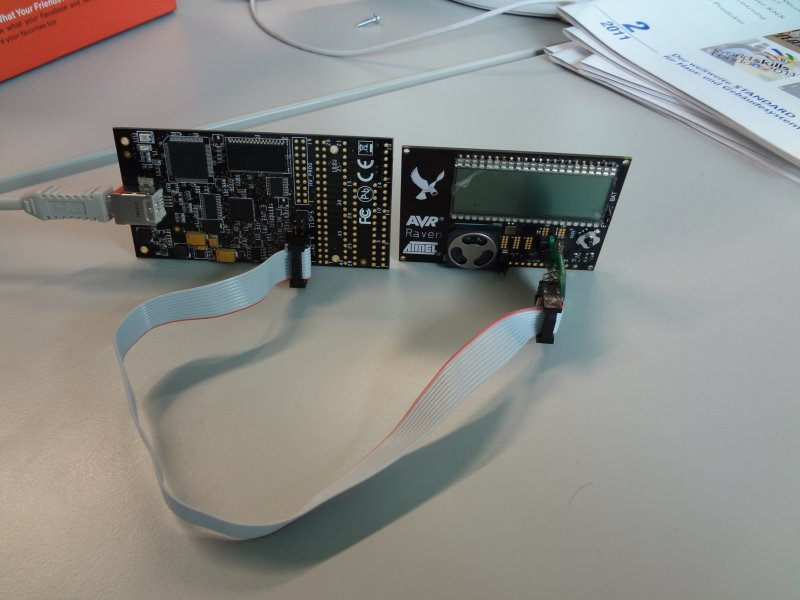
\includegraphics[width=12cm,keepaspectratio]{smallfig/DSC02184-small.jpeg}
  \caption{JTAG connected AVR Dragon to ATmega1284P CPU}
\end{figure}
Since we are using the AVR Dragon with JTAG, we need to inform the avrdude programmer about it.
Edit {\it{Makefile}} and append the following line at the bottom of the file:
\begin{lstlisting}
AVRDUDE_PROGRAMMER := -c dragon_jtag
\end{lstlisting}

This appends {\it{-c dragon\_jtag}} parameter to avrdude programmer, so it knows we are using Dragon with JTAG connected to AVR Raven.
Now we can upload the file to AVR Dragon hardware:
\begin{lstlisting}
upload compiled project using avrdude (issue as root if udev was not configured as above):
	&\textdollar& make hello-world.u
\end{lstlisting}
After successful upload we should have a running hello-world project on AVR Raven device.


\section{Network communication}
NOTE: Some of the following commands must be issued by root or with sudo. We assume sudo is configured on the system.

Assuming we have RZ USB stick and the working hello-world project,
we can setup the webserver-ipv6-raven project from Contiki examples.

As first, we need to flash the RZ USB stick to work as an Ethernet interface.

There is no widely available 802.15.4 and 6LoWPAN stack for PCs.
As a temporary solution and to be able to interconnect IPv6 hosts such as AVR Raven to IP networks,
Contiki implemented a translating function on the RZ USB Stick.
The RZ USB stick translates 802.15.4 packets to Ethernet (The Ethernet interface is emulated on the USB port).
Such a combination of this Contiki firmware and RZ USB Stick is called {\it{Jackdaw}}.


%----#--SETUP RZ USB stick connection + firmware + Photos -> HTML
Compile the project to allow RZ USB stick work as Ethernet interface:
\begin{lstlisting}
	&\textdollar& cd contiki/examples/ravenusbstick
	&\textdollar& make TARGET=avr-ravenusb
\end{lstlisting}

\begin{figure}[H]
  \centering
  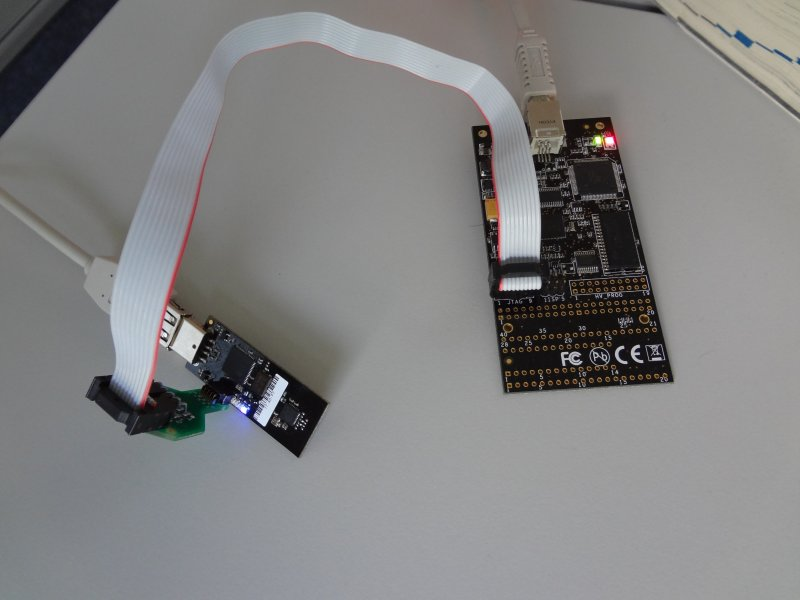
\includegraphics[width=9cm,keepaspectratio]{smallfig/DSC02595-small.jpeg}
  \caption{JTAG connected AVR Dragon to RZ USB Stick}
\end{figure}
Connect the RZ USB Stick with AVR Dragon and flash the RZ USB stick - We need to do it manually because this project does not have the upload target:
For manual flashing we need a hex file and eeprom file. The hex file should be created by Contiki automatically and called ravenusbstick.hex.
If not, we can extract it from the binary elf file:
\begin{lstlisting}
	&\textdollar& avr-objcopy -R .eeprom -R .fuse -R .signature -O ihex ravenusbstick.elf ravenusbstick.hex
\end{lstlisting}
Next we need the eeprom file. Extract it by issuing the following:
\begin{lstlisting}
	&\textdollar& avr-objcopy -j .eeprom --set-section-flags=.eeprom="alloc,load" --change-section-lma .eeprom=0 -O ihex ravenusbstick.elf ravenusbstick.eeprom
\end{lstlisting}
Assuming we have setup udev we can flash the hardware as non-root user: %!TODO UDEV FOR RZ USB STICK
\begin{lstlisting}
	&\textdollar& avrdude -u -p usb1287 -c dragon_jtag -v -P usb -Uefuse:w:0xFF:m -Uhfuse:w:0x99:m -Ulfuse:w:0xE2:m -Ueeprom:w:ravenusbstick.eeprom -Uravenusbstick.hex
\end{lstlisting}

Connect the RZ USB stick to PC and check if the network interface establishes.
\begin{lstlisting}
	&\textdollar& ifconfig
\end{lstlisting}

We should see interface called usb0 and it should get automatically IPv6 link local address, i.e. fe80::0012:13ff:fe14:1516/64.
If not add it manually:
\begin{lstlisting}
	&\textdollar& sudo ip -6 address add fe80::0012:13ff:fe14:1516/64 scope link dev usb0
\end{lstlisting}
Next we assign this interface IPv6 address and route for the whole subnet.
\begin{lstlisting}
our PC gets aaaa::1 IPv6 address:
	&\textdollar& sudo ip -6 address add aaaa::1/64 dev usb0
traffic to aaaa::/64 network goes through usb0 (RZ USB stick) interface:
	&\textdollar& sudo ip -6 route add aaaa::/64 dev usb0
\end{lstlisting}
Various parameters of RZ USB Stick, such as 802.15.4 channel,
can be configured by through /dev/ttyACM{\it{n}} character device %! TODO how does it look
accessible e.g. using the {\it{screen}} terminal emulator.


Next thing is to setup Router Advertisement Daemon (radvd), so that the Contiki node connects automatically to our IPv6 network.
Insert this configuration to {\it{/etc/radvd.conf}} or any other configuration file radvd uses.
\begin{lstlisting}
interface usb0
{
    AdvSendAdvert on;
    AdvLinkMTU 1280;
    AdvCurHopLimit 128;
    AdvReachableTime 360000;
    MinRtrAdvInterval 100;
    MaxRtrAdvInterval 150;
    AdvDefaultLifetime 200;
    prefix aaaa::/64
    {
        AdvOnLink on;
        AdvAutonomous on;
        AdvPreferredLifetime 4294967295;
        AdvValidLifetime 4294967295;
    };
};
\end{lstlisting}
Before starting radvd we must enable forwarding for IPv6:
\begin{lstlisting}
	&\textdollar& sudo sysctl -w net.ipv6.conf.all.forwarding=1
\end{lstlisting}
Now we can start the radvd - this should be done in the same way as other daemons are started on your OS.
The path might be {\it{/etc/rc.d/radvd}}, {\it{/etc/init.d/radvd}}, {\it{/usr/local/etc/rc.d/radvd}}
or any other helper script ({\it{service}}, {\it{systemctl}}, ...) can be used.
\begin{lstlisting}
	&\textdollar& sudo /etc/init.d/radvd start
\end{lstlisting}

Now we have radvd running, we can use Wireshark to check if Router Advertisement packets are being sent on usb0 interface.


Next we can setup the Contiki project and flash it to AVR Raven.

Navigate to webserver-ipv6-raven project and compile it for AVR Raven hardware:
\begin{lstlisting}
	&\textdollar& cd contiki/examples/webserver-ipv6-raven
	&\textdollar& make TARGET=avr-raven
\end{lstlisting}


The last thing is flashing our compiled binary file to AVR Raven. We need to do it manually because this project does not have the upload target.
As before we need hex and eeprom file for flashing:
\begin{lstlisting}
	&\textdollar& avr-objcopy -R .eeprom -R .fuse -R .signature -O ihex webserver6-avr-raven.elf webserver6-avr-raven.hex
	&\textdollar& avr-objcopy -j .eeprom --set-section-flags=.eeprom="alloc,load" --change-section-lma .eeprom=0 -O ihex webserver6-avr-raven.elf webserver6-avr-raven.eeprom
\end{lstlisting}
Now we can flash the hardware (use sudo if udev is not configured):
\begin{lstlisting}
	&\textdollar& avrdude -c dragon_jtag -P usb -p m1284p -Ueeprom:w:webserver6-avr-raven.eeprom -Uflash:w:webserver6-avr-raven.hex
\end{lstlisting}


If for some reason you need to specify a MAC address of the AVR Raven, you can do it by
a) setting the compile flags in Makefile before the CONTIKI directory is specified
\begin{lstlisting}
	CFLAGS+=-DMAC_ADDRESS="{0x02, 0x11, 0x22, 0xff, 0xfe, 0x33, 0x44, 0x66}"
\end{lstlisting}
and issuing make clean and compiling and flashing again
or
b) editing file contiki/platform/avr-raven/contiki-raven-main.c,
issuing make clean and compiling and flashing again.

Finally we can ping the AVR Raven and use the webserver running on it:
\begin{lstlisting}
the actual IPv6 address can be determined from Wireshark or radvd output:
	&\textdollar& ping6 aaaa::0011:22ff:fe33:4455
use wget for http communication or any other web browser:
	&\textdollar& wget --no-proxy http://[aaaa::0011:22ff:fe33:4455]
\end{lstlisting}


If you desire more information on working with AVR Raven please consult
Contiki wiki page for AVR Raven - \url{http://www.sics.se/contiki/wiki/index.php/Avr_Raven}
Contiki documentation that can be generated from source code
by issuing {\it{make}} command in {\it{doc}} directory.
\end{document}
